% generated by plots/fig4_rota.py --- do not edit the numbers by hand
% figure* --- the chapter is two-column and this does not fit one
\begin{figure*}[tp]
\centering
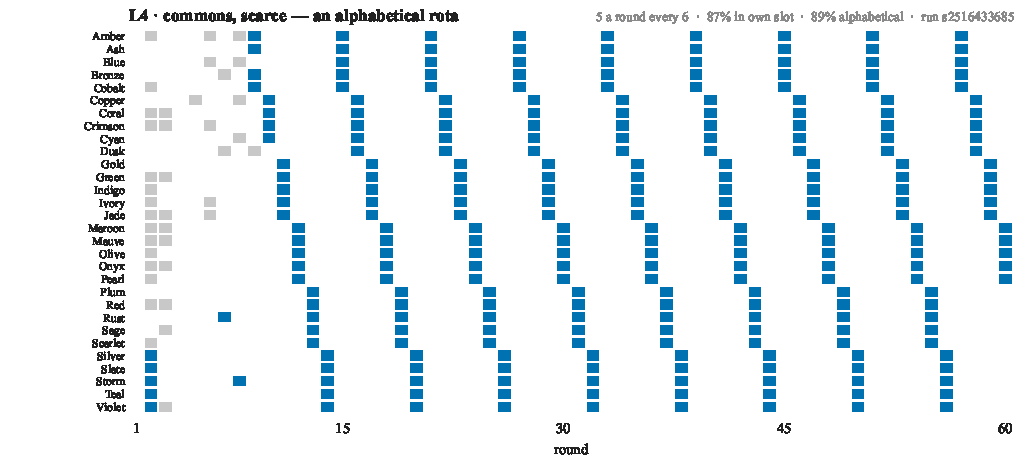
\includegraphics[width=\linewidth]{figures/fig4_rota/alphabetical.pdf}\\[2pt]
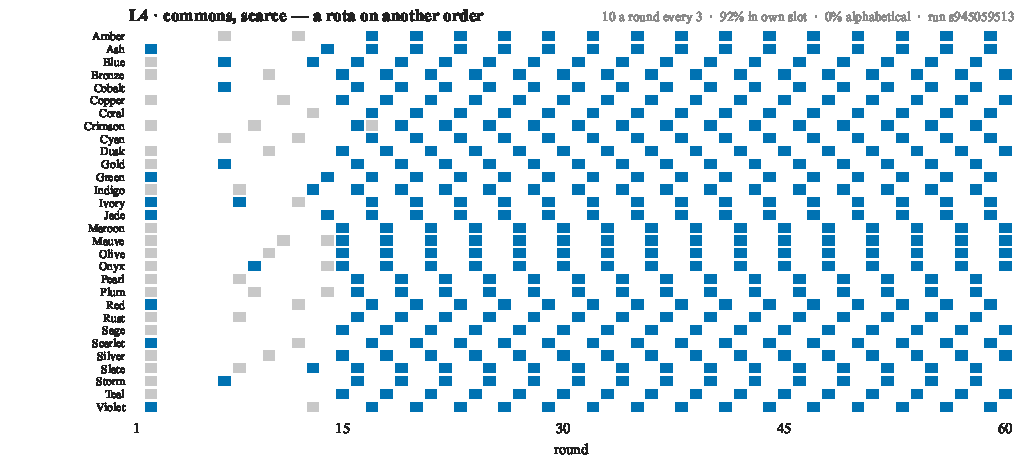
\includegraphics[width=\linewidth]{figures/fig4_rota/other_order.pdf}\\[2pt]
\caption[The rota nobody agreed]{%
\textbf{The rota nobody agreed.} Thirty agents in alphabetical order against sixty rounds, with a mark where that agent harvested in that round, drawn in colour where the harvest fell in the agent's own slot, so the grey opening of each panel is the rounds before the schedule settles and the colour is the schedule running. Both panels are the L4 scarce cell and both are rotas: run \texttt{s2516433685}, 89\% of 57 harvest rounds, 5 agents a round every 6 rounds; run \texttt{s945059513}, 0\% of 55 harvest rounds, 10 agents a round every 3 rounds. In each the population divides exactly into cohorts, harvesters a round times the period equalling the thirty agents, and once an agent has a slot it keeps it. What differs is the order the turns are taken in, since the upper panel's cohorts are blocks of the agent list while the lower panel's are drawn from across it \meth{m:harvest-rhythm} \meth{m:commons-capacity-level}.}
\label{fig:rota}
\end{figure*}
